\documentclass{neu_handout}
\usepackage{url}
\usepackage{amssymb}
\usepackage{amsmath}
\usepackage{marvosym}
\usepackage{graphicx}
\graphicspath{ {images/} }
\everymath{\displaystyle}

% Professor/Course information
\title{Update 2}
\author{Emily Dutile, Vyshaal Narayanam, Xiwen Song, Yu Tian}
\date{November 2017}
\course{CS6220}{Data Mining Techniques}

\begin{document}

\section*{1 Introduction and Background}
Today we live in a society where businesses are greatly impacted by customer reviews. For some businesses, this can greatly impact their success or failure. Looking to improve the
experience for restaurant owners and customers, we used the Yelp Open Dataset\footnote{\url{https://www.yelp.com/dataset}} that is filled with restaurant reviews of diverse content and topics, along with how a customers experience was positively or negatively impacted. Through the implementation of several data mining and text mining techniques, we can better understand user reviews and gain new insights into neighborhood businesses. In this project we mine a copious amount of Yelp restaurant reviews to address the following questions: What topics are discovered frequently in reviews and do they correlate to a positive or negative review? What neighborhoods, if any, have the best selection for a particular cuisine in a certain city? Are there some areas in a city that are more upscale or divey than others? Based upon user reviews in a particular city, can we recommend a particular dish at a top restaurant?

\subsection*{1.1 The Data}
The Yelp SQL dataset contains 4.7 million reviews, 156,000 business, and 12 metropolitan areas. Spanning over 10 years of Yelp reviews and 50 states, including international countries, the dataset provides a countless number of questions to be asked. The schema\footnote{\url{https://www.yelp.com/dataset/documentation/sql}} consists of multiple tables including information about businesses, reviews, users, checkins and tips. Since we are familiar with Boston neighborhoods and its cuisines, we wanted to find a city that we thought may have some of the same characteristics. For example, the North End in Boston is known for its Italian food and South Boston is famous for it's Irish heritage and pubs. Since Boston is not in this dataset, the majority of the project focuses on restaurants in Pittsburgh, PA, due to its relatively similar characteristics. Although it has the neighborhood Bloomfield which is equivalent to our Italian North End, it's 

As seen in Figure 1, Pittsburgh is one of the leading cities with respect to its number of restaurants and has many restaurants within close proximity of one another as seen in Figure 2. The heat map of restaurants in Pittsburgh shows that a lot of the neighborhood restaurants in the center of the city are more popular.

\begin{center}
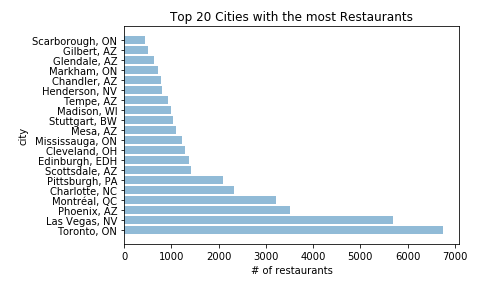
\includegraphics[width=90mm,scale=0.5]{cities}
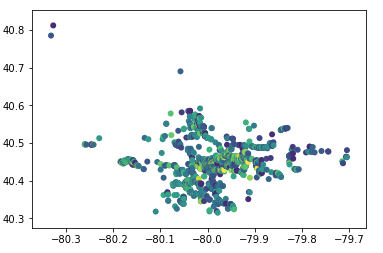
\includegraphics[width=75mm,scale=0.5]{pa_popular_restaurants}
\end{center}

Pittsburgh has 2089 restaurants, 53 different neighborhoods, and a diverse cuisine selection (43 different cuisines), which made it an interesting U.S. city to us.

The team setup local databases using PyCharm and MySQLServer in order to run faster queries. For understanding and reproducibility, the project repository and development environment set up instructions can be found on Github\footnote{\url{https://github.com/emily-jean/yelp-data-mining}}.


\subsection*{1.2 Methods}

To answer our questions, we performed data analysis and unsupervised machine learning techniques such as clustering, topic modeling and recommendation. With respect to language processing, tokenization, filtering, lemmatization, and stemming were all used for preprocessing the reviews. To tell if a customer has positive or negative feedback about a restaurant, sentimental analysis was performed in order to see if there is an interesting difference between reviews and ratings although a review is associated with a rating.


\section*{2. Exploratory Analysis}

To better visualize and explore the Pittsburgh neighborhoods a bit more, we discovered the top 10 neighborhoods with the most restaurants. Looking at other outside articles\footnote{url{https://www.thrillist.com/eat/pittsburgh/best-neighborhoods-in-pittsburgh-for-dining-and-eating-out-ranked}}, every one of these neighborhoods are listed as one of the "Best Neighborhoods for Eating" except for Oakland. The second map on the right shows the top 10 neighborhoods with the highest average review count to give some insight as to what neighborhoods are the most popular among Yelp reviewers. In comparison to the Thrillest article, only Lawrenceville, Regent Square, Shadyside, and the Strip District are on their list.

\begin{center}
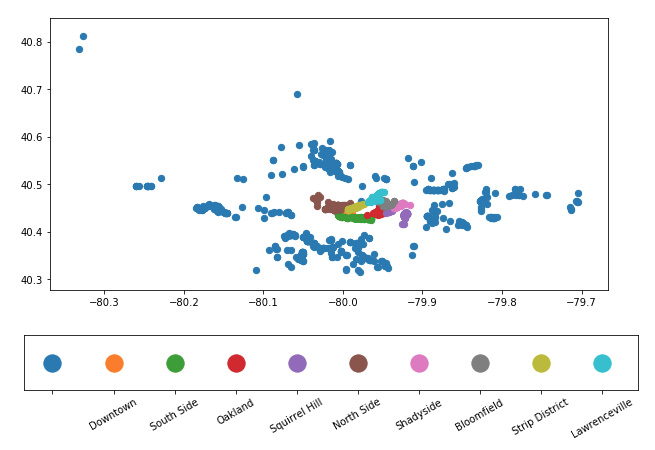
\includegraphics[width=75mm,scale=0.5]{pitts_hoods_most_restaurants}
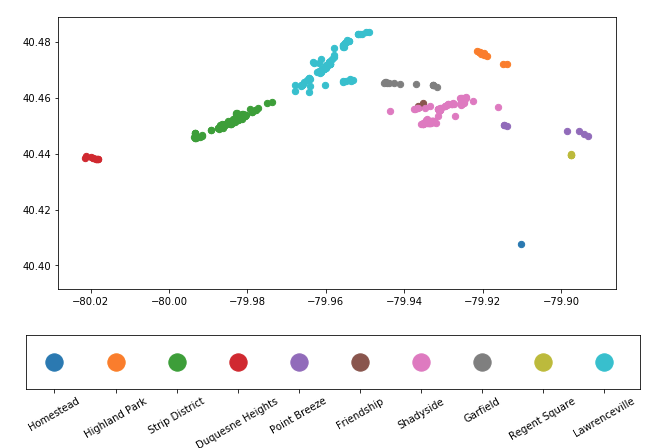
\includegraphics[width=75mm,scale=0.5]{top_10_most_popular_neighborhoods}
\end{center}

To get started on a deeper exploratory analysis of reviews and ratings, we plotted the distribution of the ratings for all the restaurants in Pittsburgh. From this plot we can see that most restaurants have a rating between 3 and 5. The average rating for Pittsburgh restaurants is 3.51. To gain a deeper insight of the data, we plotted the rating distribution of different cities. 

\begin{center}
	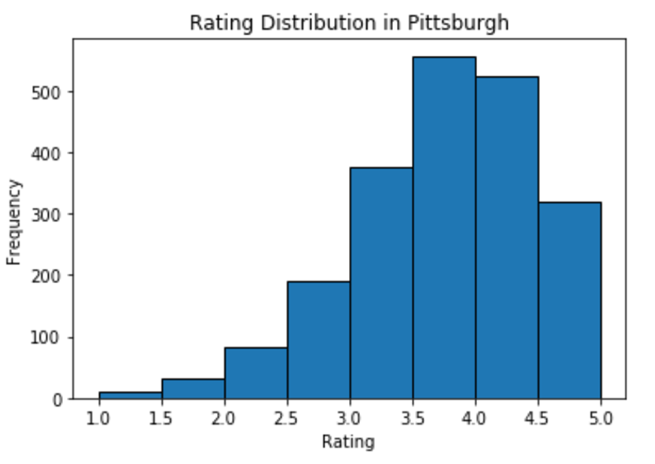
\includegraphics[width=65mm,scale=0.3]{rating_distribution_in_Pittsburgh}
	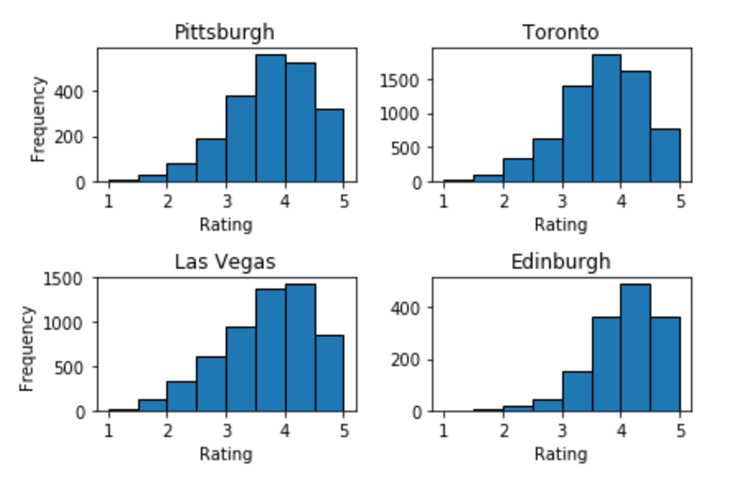
\includegraphics[width=75mm,scale=0.3]{rating_distribution_vs_countries}
\end{center}

Besides looking at the basic distribution, we plotted the relationship between the average number of reviews and rating level using box plot. Our original belief was that we thought better restaurants should receive more reviews. However, the results show us that restaurants with a medium rating acquire more reviews. 

\begin{center}
	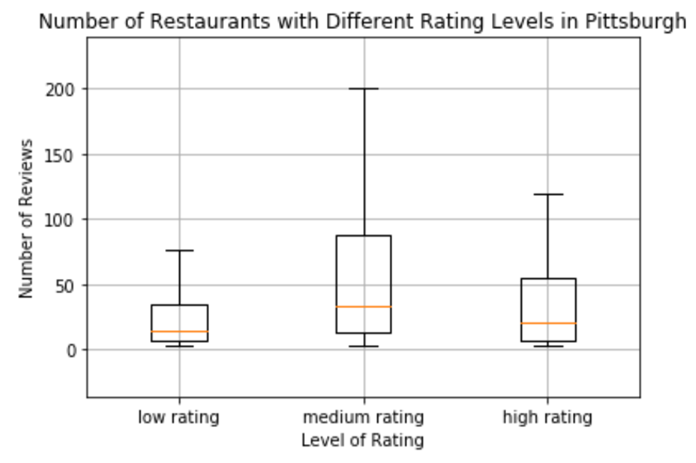
\includegraphics[width=75mm,scale=0.3]{number_of_restaurants_vs_rating_level}
\end{center}

We also explored the relationship between average number of reviews, the average length of review (after tokenization and stemming) and each cuisine. In Pittsburgh in appears that Japanese foods receive the most reviews while Chinese foods receive the least number of reviews. When looking at the length of review, there doesn't appear to be many differences among the variety of cuisines. 

\begin{center}
	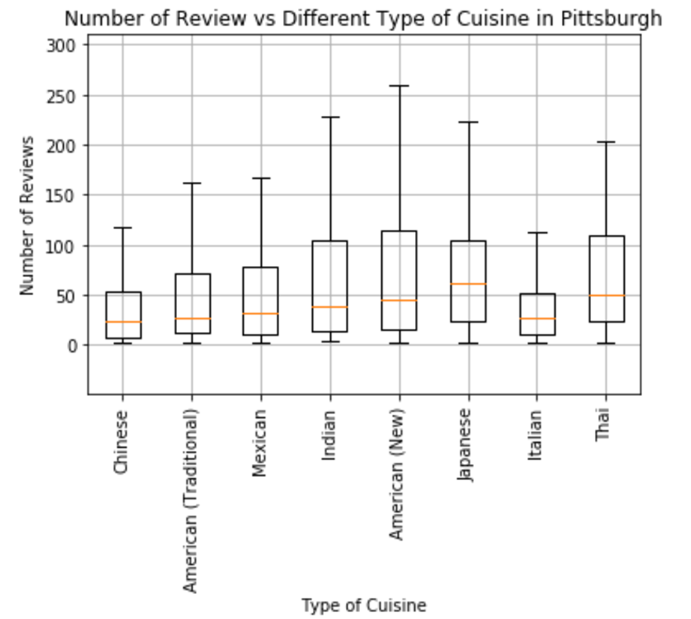
\includegraphics[width=75mm,scale=0.3]{number_of_review_vs_cuisine}
	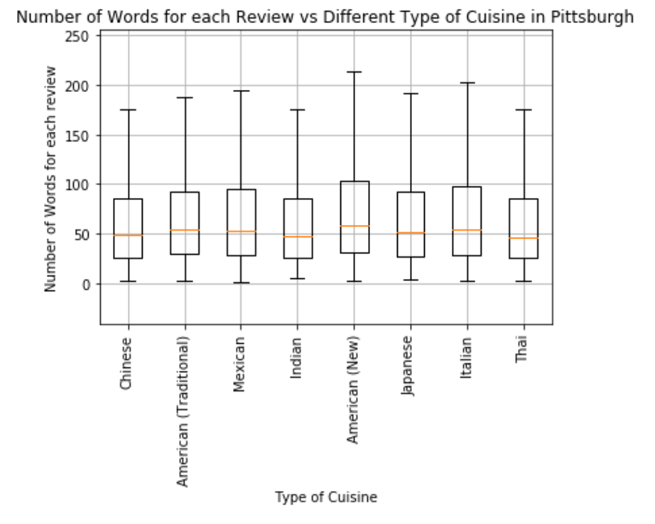
\includegraphics[width=85mm,scale=0.3]{average_review_length}
\end{center}

Furthermore, to get a better sense on how the contents of a review correlate with the rating, we calculated the ratings for one of the restaurant by performing sentiment analysis on the reviews and then comparing the results with the dataset ratings. Through sentiment analysis, we can determine whether the review is positive or negative. We took a sample dataset of all restaurants in Pittsburgh which have more than 200 reviews to assign our own ratings (there are 109 restaurants in Pittsburgh which satisfy our criteria), and computed the average of the values obtained from sentiment analysis of all the reviews (38,785 reviews) of that restaurant. The sentimental analysis is done using PatternAnalyzer in nltk (textblob is built over nltk). We assigned a weight of +5 for a positive review and -5 for a negative review. These newly derived ratings are compared with the ratings in original dataset as shown in the histogram. We can assume that these reviews are more accurate because we are incorporating negative weights to low star reviews.

\begin{center}
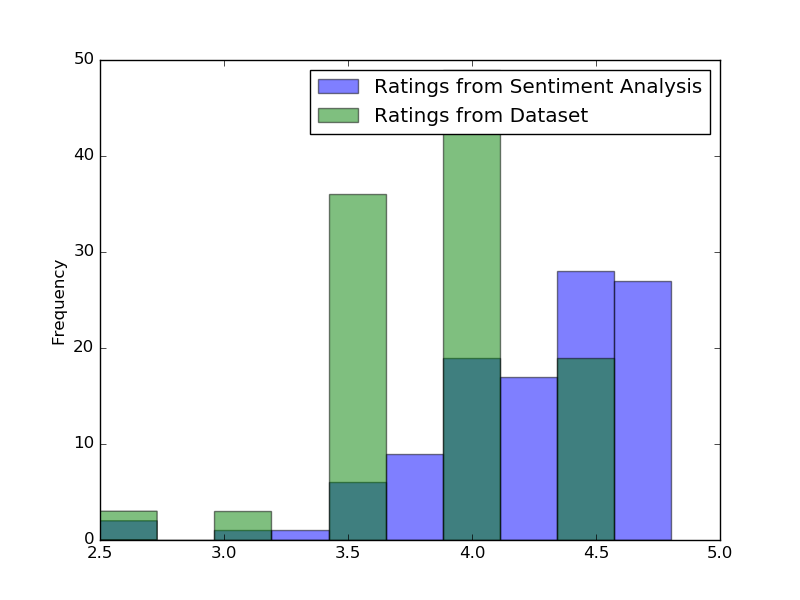
\includegraphics[width=90mm,scale=0.5]{sentimentanalysis}
\end{center}

Next, we extracted the top 50 keywords from positive and negative reviews. Again taking a sample dataset of all restaurants in Pittsburgh that have more than 200 reviews. There are a total of 38,785 reviews. Data processing techniques such as tokenizing, filtering, stemming and filtering the key words from those reviews were performed. We then calculated 50 most frequent keywords from the negative and positive reviews separately. Negative and positive reviews were distinguished using the polarity obtained in the previous step.
The results are very promising. Few keywords such as "great","good","nice","service" came with high frequency in positive reviews where as words like "bad","good","terrible","poor","great" appeared negative reviews. Common words such as "Pittsburgh", "food", "service", and "place" are present in both positive and negative reviews. One important thing to notice is that "good" and "great" appeared in negative reviews too in a sense that customers are complaining how the food isn't that good/great. The high frequencies of words in positive reviews when compared to negative reviews is because of more number of positive reviews in the corpus.

\begin{center}
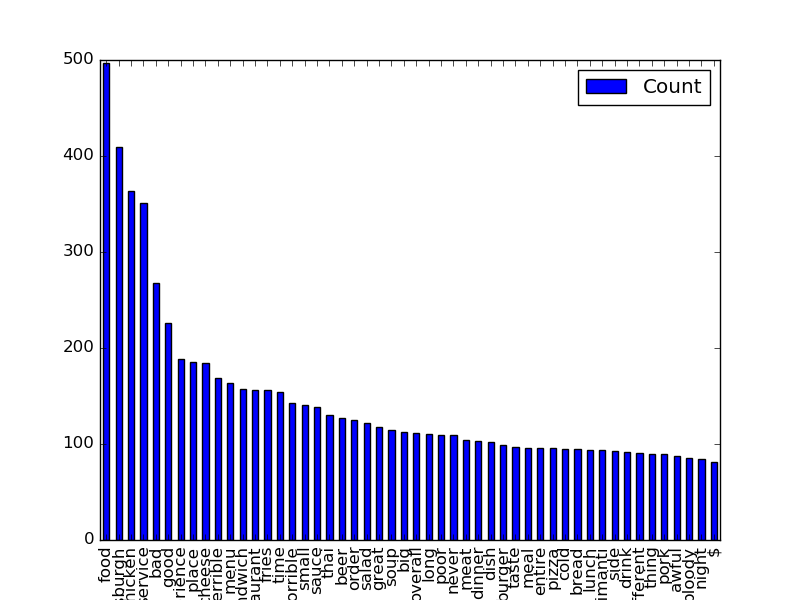
\includegraphics[width=70mm,scale=0.5]{top50_negativereviews}
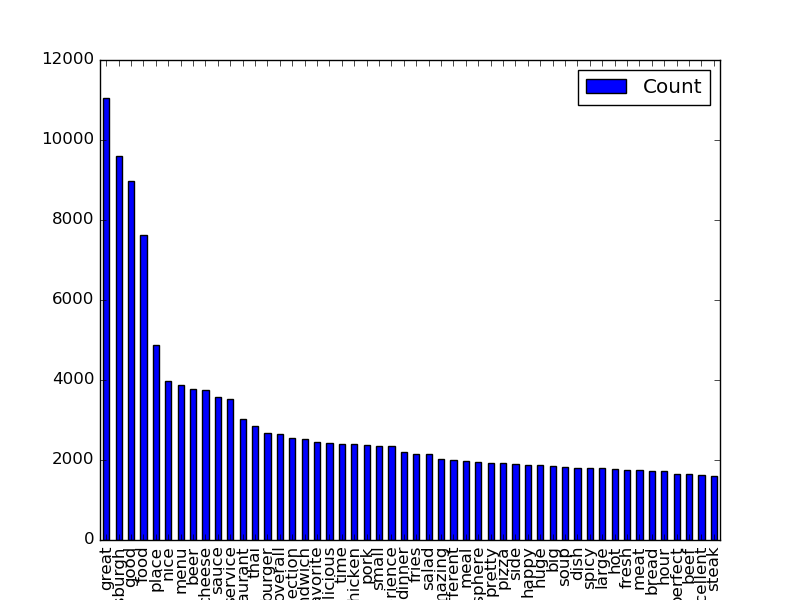
\includegraphics[width=70mm,scale=0.5]{top50_positivereviews}
\end{center}

Although some of our exploratory analysis focused on one city, we expanded our reviews analysis to 4 different cities with the most reviews (Edinburgh, Toronto, Las Vegas, and Pittsburgh), from 3 different countries. The thought here was that there may be differences between different cities such as the service, or people may have different diction. It's possible that the final cluster may be verified by different external evaluation criteria, so we thought it'd be useful to further explore this area. We plotted the differences of rating habits among the 4 cities based on average rating score for each type of cuisine. Edinburgh has the best rating feedback, relatively speaking, while Toronto seems to be lacking Yelper feedback.

\begin{center}
	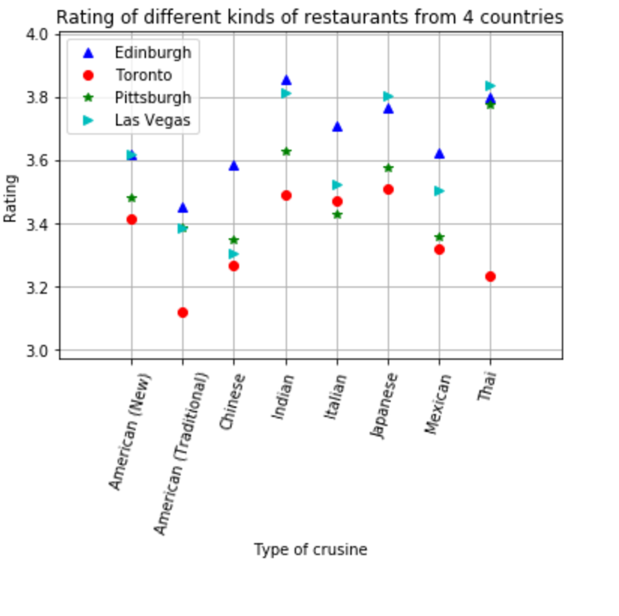
\includegraphics[width=60mm,scale=0.5]{Rating_different_restaurants_countries.png}
\end{center}

\section*{3 Data Mining Analysis}

To find what cuisines may lie in particular neighborhoods in Pittsburgh, we performed two clustering techniques: K-Means++ and GMM. In order to do this, we decided to look at the closeness and similarities of the restaurants by using the longitude and latitude which considered cluster closeness, as well as the category/cuisines to cluster for similarity. During the data exploration, we intentionally dug into all the types of categories, realizing that we would want to filter out other non-restaurant businesses as well as things such as 'cafe' or 'breakfast' which we didn't identify as a cuisine. This left us with a list of 49 cuisines and didn't consider any cuisine that had less than 10 restaurants. The SQL data was parsed into a pandas dataframe which has two columns for latitude and longitude, and the remaining are all the cuisines in Pittsburgh. If a restaurant is of that cuisine then the value for the column is 1 (else 0). Through subtracting the mean of the whole column from each value, dividing that by the standard deviation in order to get the z-score, feature scaling was performed on longitude and latitude in order to scale down the location to a range of cuisines. We selected 5 to be the appropriate number of clusters for KMeans++ by creating a plot to show the error vs. the number of clusters since it appears to be the greater 'bend' in the elbow. 

\begin{center}
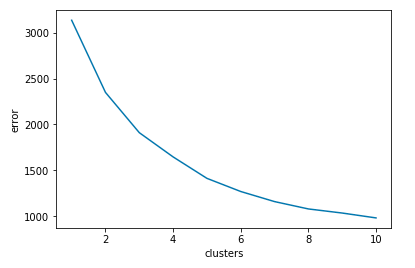
\includegraphics[width=70mm,scale=0.5]{kmeanserror}
\end{center}

With the GMM implementation, we use co-variance as 'spherical' so that each component has its own single variance. As since in the figures below, the longitude/latitude of the restaurants have been plotted and each cluster is labeled with a cuisine. In order to avoid dominance of a particular cuisine purely because the number of restaurants it has in Pittsburgh, we calculated the ratio of each cuisine in the cluster with the total number of restaurants in that category, and then selected the category that has the maximum ratio to be the cluster label.

\begin{center}
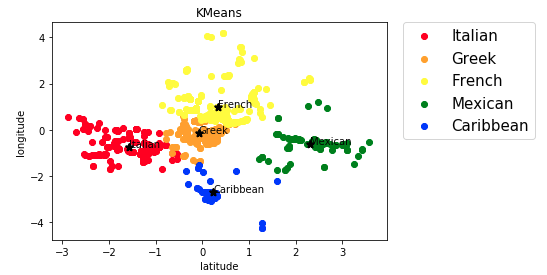
\includegraphics[width=70mm,scale=0.5]{kmeans}
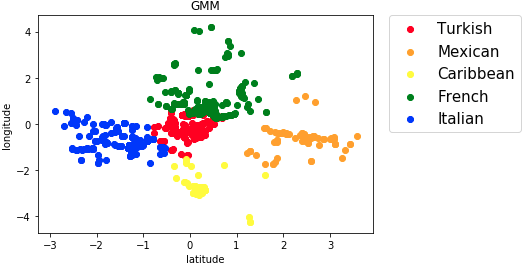
\includegraphics[width=70mm,scale=0.5]{gmm}
\end{center}


\section*{4 Discussion}

Looking at the overall results of our data analysis and implementation, the group was pleasantly surprised by the outcomes.

With our original intention to cluster cuisines by neighborhoods, K-Means had more well-defined clusters since each point only belongs to one cluster. On the other hand, GMM has over-lapping clusters since it calculates the probability of a point belonging to each cluster and therefore seemed to give better clustering.


\section*{5 References}




\end{document}
